%%%%%%%%%%%%%%%%%%%%%%%%%%%%%%%%%%%%%%%%%
% Rapport sur package R6
% Version 1 (14/11/2024)
%
% Auteurs :
% Linh Nhi Le Dinh
% Antoine Oruezabala
% Béranger Thomas
%
%%%%%%%%%%%%%%%%%%%%%%%%%%%%%%%%%%%%%%%%%

%----------------------------------------------------------------------------------------
%	Packages
%----------------------------------------------------------------------------------------

% Classe du document
\documentclass[10pt,french]{report}

% Packages langue française
\usepackage[frenchb]{babel}
% Pour les guillemets en style français
\usepackage[french=guillemets]{csquotes}

% Saisir des caractères spéciaux et accentués
\usepackage[utf8]{inputenc}
% Imprimer des caractères spéciaux et accentués
\usepackage[T1]{fontenc}

% Améliorer les espacements
\usepackage{microtype}

\usepackage[a4paper, portrait]{geometry}

% Pour faire des tableaux plus efficacement
\usepackage{tabularray}

% Pour les symboles des équations mathématiques
\usepackage{mathtools}
\usepackage{amssymb}

% Pour charger et afficher des images
\usepackage{graphicx}
\graphicspath{{images/}}


% Pour représenter l'arborescence du programme
\usepackage{dirtree}


% Gérer les espaces entre paragraphes plus facilement
\usepackage{parskip}
\setlength\parindent{0pt}


% Polices de caractères
\usepackage{lmodern}
%\usepackage{stix2} % font stix 2
\usepackage{palatino} % font Palatino


% Pour créer des conditions dans les commandes customisées
\usepackage{ifthen}


% Commande customisée pour dessiner un cube noir, pour faire séparateur
\newcommand{\cube}{\raisebox{0.13ex}{\scalebox{0.75}{ $\blacksquare$ }}}


% Commande customisée pour les entrées du lexique
\newcommand{\entreelex}[3][]{%
	{\large \textbf{\textsc{#2}}} % Entrée (obligatoire)
	\if\relax\detokenize{#1}\relax % Si #1 est vide
	\else % Si #1 n'est pas vide
	\raisebox{0.15ex}{\scalebox{0.7}{$\Diamond$}} % Diamant
	[#1] % Acronyme (facultatif)
	\fi
	\raisebox{0.13ex}{\scalebox{0.75}{$\blacksquare$}} #3 % Définition (obligatoire)
}


% Bibliographie : sous TexStudio, faire F5, puis F8, puis F5 à nouveau (c'est Latex, c'est tout simple)
\usepackage[style=numeric]{biblatex}
\addbibresource{Rapport.bib}


% Pour faire des hyperliens
\usepackage[colorlinks=true, linkcolor=NavyBlue]{hyperref}
% et leur donner une couleur plus sympa que le bleu habituel
\usepackage[dvipsnames]{xcolor}
\hypersetup{colorlinks=true, citecolor=NavyBlue}

%----------------------------------------------------------------------------------------

\begin{document}

	\begin{titlepage}
		\centering
		\includegraphics[width=0.6\textwidth]{icom.png}\par\vspace{0.5cm}
		{\Large\bfseries Université Lumière Lyon 2}\par
        \par\vspace{3.5cm}



		{\Huge\bfseries Librairie MIMOSA}\par\vspace{0.75cm}
		{\huge\bfseries Mixed Input Multinomial Optimization for Statistical Analysis}\par\vspace{0.75cm}

		{\Large\itshape Régression logistique multinomiale sur données mixtes,\\par descente de gradient}\par\vspace{3.5cm}

		{\Large\itshape Par}\par
		{\Large Linh Nhi Le Dinh}\par
		{\Large Antoine Oruezabala}\par
		{\Large Béranger Thomas}\par\vspace{1cm}

		{\large\itshape Rapport présenté dans le cadre du}\par
		{\large Master 2 SISE - Promotion 2024/2025}\par\vspace{1cm}

		\vfill

	\end{titlepage}

	\tableofcontents

	\setlength{\parskip}{12pt}

	\begin{abstract}
		Ce rapport détaille l'implémentation de la régression logistique multinomiale pour des données mixtes, en langage R, et en utilisant la descente de gradient. Nous couvrons tout d'abord quelques fondements théoriques, puis l'approche pratique et enfin discutons des résultats obtenus. En fin d'ouvrage, une bibliographie donnera quelques pistes au lecteur curieux d'approfondir certains aspects, ou désireux d'apprendre par le biais d'une pédagogie quelque fois différente de celle de ce rapport. Un lexique vient également compléter nos écrits et donne accès à des définitions et formules mathématiques de façon plus condensés que dans le corps du texte.

		Ce rapport a été rédigé en novembre 2024 dans le cadre d'un projet du master 2 SISE.
	\end{abstract}

	\chapter{Théorie}

	\section{La régression logistique multinomiale}
	\subsection{Principes Généraux}
	% Description du modèle multinomial et de ses applications.
	La régression logistique est un modèle statistique permettant d'étudier les relations entre un ensemble de variables Xi et une variable qualitative y. Elle permet de prédire la probabilité qu'un événement arrive (valeur de 1) ou non (valeur de 0) à partir de l'optimisation des coefficients de régression.

	On distingue trois types de régression logistique :
	\begin{enumerate}
		\item La régression logistique binaire. Elle vise à prédire la probabilité qu'un événement binaire se produise (oui/non, 1/0) en fonction de variables explicatives. Elle utilise la fonction sigmoïde pour transformer la combinaison linéaire des variables explicatives en une probabilité comprise entre 0 et 1.
		\item La régression logistique \textbf{multinomiale} est une généralisation de la régression logistique binaire. Elle permet d'estimer la probabilité d'appartenance à chacune des catégories en fonction de variables explicatives quantitatives et/ou qualitatives. Contrairement à la régression logistique binaire qui modélise une seule probabilité $p$, la régression logistique multinomiale estime simultanément les probabilités d'appartenance à toutes les catégories ($p_1, p_2, ..., p_K$) avec la fonction softmax, et avec la contrainte que leur somme soit égale à 1.
		\item La régression logistique ordinale. Ce type de modèle de régression logistique est utilisé lorsque la variable de réponse a trois modalités possibles ou plus et que ces dernières ont un ordre défini.
	\end{enumerate}

	Dans ce document, nous ne supposerons aucun ordre particulier entre les modalités de la variable à prédire.

    \subsection{Modélisation mathématique\cite{makisreglog}}

    \subsubsection{Notations}

    Soit une population $\Omega$ de $n$ individus, définie par $J$ variables explicatives notées $\left\{X_{1}, \ldots,X_{J}\right\}$, et une variable cible $Y$ possédant $K$ valeurs :

    \begin{tblr}{
            colspec = {X[4,c]X[4,c]X[4,c]X[4,c]X[4,c]},
            rowspec = {Q[m]Q[m]Q[m]Q[m]Q[m]},
            rowsep = 5pt,
            hlines,
            vlines,
        }
        $\Omega$ & Cible & $X_{1}$ & $\ldots$ & $X_{J}$ \\
        1 & $Y_{1}$ &  &  &  \\
        $\ldots$ & $\ldots$ &  &  &  \\
        $\omega$ & $Y_{\omega}$ & $X_{1}\left(\omega\right)$ & $\ldots$ & $X_{J}\left(\omega\right)$ \\
        $\ldots$ & $\ldots$ &  &  &  \\
        $n$ & $Y_{K}$ &  &  &  \\
    \end{tblr}

    Dans le cas binaire, la probabilité d'un individu $\omega$ d'être positif à priori se note $p$ par commodité, pour simplifier $p\left(\omega\right)$, lui-même une notation simplifiée de $P\left[Y\left(\omega\right)=+\right]$.

    Toujours dans le cas binaire, la probabilité d'un individu $\omega$ d'être positif à posteriori, c'est-à-dire la probabilité que l'on modélisera en apprentissage supervisée, se note $\pi$ par commodité, pour simplifier $\pi\left(\omega\right)$, lui-même une notation simplifiée de $P\left[Y\left(\omega\right)=+/X\left(\omega\right)\right]$.

    La fonction LOGIT pour cet individu $\omega$ est :

    \begin{equation}
        \text{LOGIT}(\omega) = \ln\left[\frac{\pi(\omega)}{1-\pi(\omega)}\right] = a_0 + a_1X_1\left(\omega\right) + \cdots + a_JX_J\left(\omega\right)
    \end{equation}

    Soit en écriture matricielle :

    \begin{equation}
        \ln\left[\frac{\pi(\omega)}{1-\pi(\omega)}\right] = X\left(\omega\right) \times a
    \end{equation}

    Avec $a_0, \ldots, a_J$ les paramètres que l'on souhaite estimer.

    \subsubsection{Formulation du problème}

    Soit :
    \begin{itemize}
    	\item $Y$ une variable catégorielle cible prenant $K$ valeurs distinctes : $\{1, 2, \dots, K\}$,
    	\item $X$ est un vecteur des $p$ variables explicatives pour une observation donnée,
    	\item $\boldsymbol{\beta}_k$ est un vecteur des coefficients associés à la classe $k$,
    	\item $P(Y = k \mid X = \mathbf{x})$ est la probabilité conditionnelle pour chaque classe $k \in \{1, 2, \dots, K\}$.
    \end{itemize}

    \subsubsection{Colinéarité}

    Pour éviter les problèmes de colinéarités, on choisit une classe de référence que l'on exclut de la modélisation.

    Les probabilités des $k-1$ classes se calculent avec :

    \begin{equation}
    	P_k = \frac{e^{C_k}}{1+\sum_{k=1}^{K-1}e^{C_k}}
    \end{equation}

    Avec $C_k$ le logit pour la modalité $k$ de $Y$; et comme indiqué précédemment $k \in \{1, 2, \dots, K-1\}$.

    La probabilité pour la classe de référence $K$ peut être déduite après coup :

    \begin{equation}
    	P_K = 1 - \sum_{k=1}^{K-1}P_k
    \end{equation}

    \section{La descente de gradient}

    L'estimation des coefficients $\beta$ peut se faire par descente de gradient.

    La descente de gradient est un algorithme d'optimisation itératif, qui permet de trouver le minimum d'une fonction.

    L'idée est la suivante :
    \begin{itemize}
    	\item on part d'un point choisi aléatoirement,
    	\item depuis ce point nous cherchons le gradient (la pente),
    	\item et nous descendons d'un pas dans la direction opposé au gradient,
    	\item nous recommençons le processus à partir du nouveau point atteint.
    \end{itemize}

    Les critères pour s'arrêter peuvent être :
    \begin{itemize}
    	\item le nombre d'itérations; on définit un maximum au début de l'algorithme, que l'on ne dépasse pas,
    	\item la différence de "niveau" entre deux points; si elle passe en dessous d'un seuil très faible, l'approximation est jugée suffisamment bonne,
    	\item une combinaison de ces deux critères, qui a l'avantage de s'arrêter le plus tôt possible.
    \end{itemize}

    Vocabulaire :
    \begin{itemize}
    	\item la taille du pas est dénommé taux d'apprentissage (en anglais learning rate),
    	\item la différence minimale souhaitée entre deux points consécutifs est la tolérance,
    	\item
    	\item
    \end{itemize}

    Mathématiquement, la pente est définie par le gradient. La taille du pas est dénommé taux d'apprentissage.

    Il existe trois types d'algorithmes d'apprentissage par descente de gradient : la descente de gradient simple (sur tous les points), la descente de gradient stochastique et la descente de gradient par mini-lots.


	\subsection{Fonction de Coût}
	% Explication de la fonction d'erreur cross-entropy catégorielle.
	La fonction de coût utilisée pour la régression logistique multinomiale est la cross-entropie catégorielle. Elle évalue la divergence entre les probabilités prédites par le modèle et les probabilités réelles des classes. Elle est définie comme suit :

	\[
	J(\beta) = -\frac{1}{N} \sum_{i=1}^{N} \sum_{k=1}^{K} y_{i,k} \log\left( P(Y = k \mid X_i) \right)
	\]

	où :

	- \( N \) est le nombre total d'observations.
	- \( K \) est le nombre de classes.
	- \( y_{i,k} \) est une variable indicatrice qui vaut 1 si l'observation \( i \) appartient à la classe \( k \), et 0 sinon.
	- \( P(Y = k \mid X_i) \) est la probabilité prédite que l'observation \( i \) appartienne à la classe \( k \).

	Minimiser cette fonction de coût permet d'ajuster les paramètres \( \beta \) du modèle pour améliorer la précision des prédictions. La descente de gradient est une méthode d'optimisation utilisée pour trouver les valeurs optimales de \( \beta \) qui minimisent \( J(\beta) \).

	La fonction \textit{SoftMax} est essentielle dans ce modèle car elle transforme les scores linéaires en probabilités. Elle garantit que les sorties du modèle sont comprises entre 0 et 1 et que la somme des probabilités pour toutes les classes est égale à 1 pour chaque observation. La fonction \textit{SoftMax} est définie par :

	\[
	P(Y = k \mid X) = \frac{\exp(X\beta_k)}{\sum_{j=1}^K \exp(X\beta_j)}
	\]

	où \( K \) est le nombre total de classes. Cette transformation est basée sur l'hypothèse que les logits peuvent être exponentiés et normalisés pour obtenir des probabilités, ce qui est cohérent avec le principe de maximum d'entropie.

	L'utilisation de la fonction \textit{SoftMax} implique également que les classes sont mutuellement exclusives, ce qui signifie qu'une observation ne peut appartenir qu'à une seule classe. Cela correspond à la nature des problèmes de classification multinomiale où le but est de prédire une seule catégorie parmi plusieurs possibles.

	\section{Algorithmes de descente de gradient}

	\subsection{Modélisation}

    Il s'agit aussi d'un algorithme itératif, dont l'objectif est de trouver le minimum d'une fonction $f\left(x\right)$ en partant d'un point arbitraire $x_0$. On se \enquote{déplace} pour cela dans la direction opposée au gradient, c'est-à-dire que l'on \enquote{descend} le long de la pente.

    Mathématiquement, on part d'une valeur arbitraire $x_0$, puis pour trouver $x_1$ on utilise la formule suivante :

    \begin{equation}
        x_{n+1} = x_n - \alpha \nabla f\left(x_n\right)
    \end{equation}

    Avec :
    \begin{itemize}
        \item $x_n$ la position actuelle,
        \item $\alpha$ le taux d'apprentissage,
        \item $\nabla f\left(x_n\right)$ le gradient de la fonction au point $x_n$
    \end{itemize}

    Les étapes sont donc les suivantes :
    \begin{itemize}
        \item choisir un point $x_0$ arbitraire pour commencer les calculs,
        \item calculer le gradient à ce point,
        \item mettre à jour la position en se déplaçant dans la direction opposée,
        \item vérifier que l'on a atteint un critère d'arrêt :
        \begin{itemize}
            \item nombre d'itérations maximum atteint,
            \item ou précision souhaitée (différence entre deux itérations) atteinte,
			\item ou norme du gradient devient suffisamment petite (proche d'un point critique),
			\item ou variation des paramètres entre deux itérations devient très petite,
			\item ou utilisation de plusieurs critères simultanément pour garantir une convergence robuste.
        \end{itemize}
		\item vérifier que le point obtenu satisfait réellement les conditions nécessaires pour être un minimum local :
		\begin{itemize}
			\item la norme du gradient $(\vert \vert)\nabla f\left(x^\star\right)(\vert \vert)$ est proche de zéro, 
			\item la matrice hessienne $\nabla^2 f\left(x^\star\right)$ (si calculable) est définie positive, confirmant que $x^\star$ est un minimum local.
		\end{itemize}
		\item calculer la valeur de $f(x^\star)$ pour s'assurer qu'elle est acceptable par rapport aux exigences du problème.
        \item vérifier si la solution $x^\star$ est cohérente et utile dans le cadre du problème initial.
		\item tester la solution obtenue.
		\item si la solution obtenue n'est pas satisfaisante , des méthodes complémentaires peuvent être utilisées :
		\begin{itemize}
			\item relancer la descente de gradient à partir d'un autre point initial pour explorer d'autres minima.
			\item compléter par une recherche globale .
			\item si le critère d'arrêt a été atteint trop tôt à cause d'un pas mal adapté, réajuster les paramètres.
		\end{itemize}
    \end{itemize}

	\subsection{Test}

	Les tests permettent de quantifier la qualité d’un modèle lorsque l'on rajoute une variable supplémentaire. 

	Nous avons trois tests : 
	\begin{itemize}
		\item le test de Wald  
		\item le test du rapport de vraisemblance 
		\item le test du score de Rao 
	\end{itemize}
	
	Nous allons maintenant présenter les formules de ces tests.
	
	La statistique du test de Wald:

	\begin{equation}
		Z_j = sign(\beta_j) \cdot \frac{\beta_j}{\sigma_{\beta_j}}
	\end{equation}
	
	où $\beta_j$ désigne le coefficient estimé de la variable $X^j$ et de $\sigma_{\beta_j}$ son écart-type.

	La statistique du test suit un loi normale centrée-réduite et l’hypothèse $H_0$ est que coefficient estimé est nul.

	La statistique du test de rapport de vraisemblance:

	\begin{equation}
	D = -2 ln (\frac{\mbox{Vraisemblance modele de reference}}{\mbox{Vraisemblance modele d'interet}})
	\end{equation}

	La statistique de test suit une loi du $\chi^2$ de paramètre $(df_1 - df_2)$ où $df_k$ désigne le nombre de variables du modèle $k$. L’hypothèse $H_0$ est que les modèles sont semblables.

	La statistique du test du Score de Rao:

	\begin{equation}
	R = U_{H_0} ^T (\beta) I_{H_0} ^{-1} (\beta) U_{H_0} (\beta)
	\end{equation}

	Où $U_{H_0}$ est la matrice des dérivées partielles de la log-vraisemblance et $I$ la matrice d’information.

	La statistique de test suit une loi du $\chi ^2$ de paramètre $P$. L’hypothèse $H_0$ est que les coefficients sont nuls.

	\chapter{Implémentation Pratique en R}

	\section{Structure du programme}

	L'architecture du programme est la suivante :

	\dirtree{%
		.1 {projet\textunderscore racine/}.
		.2 {datasets/}.
		.2 {docs/}.
		.3 {Rapport.pdf}.
		.3 {Rapport.tex}.
		.2 {utils/}.
		.3 {LogisticRegression.r}.
		.3 {preprocessing.r}.
		.3 {utils.r}.
		.2 {main.r}.
	}

	Les fichiers sont décrits ci-après, avec du pseudo-code pour certaines fonctions.

	\subsection{main.r}

	Le fichier \texttt{main.r} contient le programme principal, qui instancie l'objet \texttt{LogisticRegression}, qui contient les fonctions suivantes :

	\begin{itemize}
		\item \texttt{fit} : pour modéliser
		\item \texttt{transform} : pour
		\item \texttt{probas}
	\end{itemize}

	\subsection{utils.r}

	Le fichier \texttt{utils.r} contient une fonction \textit{check\textunderscore type}, qui vérifie si l'objet passé en premier argument est du même type que le type passé en second argument.

	Si ce n'est pas le cas, le programme s'arrête.

	\subsection{preprocessing.r}

	Le fichier \texttt{preprocessing.r} contient plusieurs fonctions de prétraitement :

	\begin{itemize}
		\item imputer\textunderscore numeriques : réalise une imputation par la moyenne des valeurs manquantes dans le jeu de données passé en argument.
		\item imputer\textunderscore categorielles : réalise une imputation par le mode des valeurs manquantes dans le jeu de données passé en argument.
		\item split\textunderscore train\textunderscore test : réalise une séparation du jeu de données passé en argument
	\end{itemize}

	\subsection{LogisticRegression.r}

	Le fichier \texttt{LogisticRegression.r} contient toutes les fonctions nécessaires à la réalisation de la régression logistique :

	\subsubsection{Fonction \enquote*{sigmoid}}
	Applique la \hyperref[fonction sigmoïde]{fonction sigmoïde} à la valeur passée en argument et renvoie le résultat.

	\subsubsection{Fonction \enquote*{softmax}}
	Applique la \hyperref[fonction softmax]{fonction softmax} à la valeur passée en argument et renvoie le résultat.

	\subsubsection{Fonction \enquote*{cout}}
	Fonction de coût pour la régression logistique, avec cross-entropy :

	\begin{verbatim}
		cout <- function(X, y, beta) {
			   n <- nrow(X)
			   scores <- X %*% beta
			   probs <- exp(scores) / rowSums(exp(scores))
			   cost <- -mean(sum(y * log(probs)))
			   return(cost)
		    }
	\end{verbatim}

	\subsubsection{Fonction \enquote*{hypothese}}

	\subsubsection{Fonction \enquote*{descente\textunderscore gradient}}

	Applique une descente de gradient pour la régression logistique :
	\begin{verbatim}
		descente_gradient <- function(X, y, beta) {
			n <- nrow(X)
			scores <- X %*% beta
			probs <- exp(scores) / rowSums(exp(scores))
			gradient <- -t(X) %*% (y - probs) / n
			return(gradient)
		}
	\end{verbatim}

	\subsubsection{Fonction \enquote*{summary}}
    Affiche les informations du modèle 
    \begin{verbatim}
    	summary = function(class_names = NULL) {
      		self$print()
      		cat("\nModel Weights (if trained):\n")

      		if (!is.null(self$weights)) {
        		intercept <- self$weights[1, , drop = FALSE]  
        		coefficients <- self$weights[-1, , drop = FALSE]  

        		if (self$classification_type == "binary") {
          			weights_binary <- cbind(-self$weights, self$weights)  
          			rownames(weights_binary) <- c("(Intercept)", colnames(X_train)) 

          			weights_binary_sorted <- weights_binary[order(-abs(weights_binary[, 2])), 
          			, drop = FALSE]

          			if (!is.null(class_names) && length(class_names) == 2) {
            			colnames(weights_binary_sorted) <- class_names  
          			} else {
            			colnames(weights_binary_sorted) <- c("Class 0", "Class 1") 
          			}

          			cat("\nWeights (Binary Classification, sorted by absolute value):\n")
          			print(weights_binary_sorted)

          			feature_importance <- data.frame(
            		Feature = rownames(weights_binary_sorted)[-1],  
            		Importance = abs(weights_binary_sorted[-1, 2])  
          			)

        			} else if (self$classification_type == "softmax") {
          			if (!is.null(class_names)) {
            			colnames(self$weights) <- class_names
          			}

          			intercept <- self$weights[1, ]  
          			coefficients <- self$weights[-1, , drop = FALSE]  

          			total_importance <- rowMeans(abs(coefficients))

          			sorted_indices <- order(-total_importance)
          			coefficients_sorted <- coefficients[sorted_indices, , drop = FALSE]

          			rownames(coefficients_sorted) <- colnames(X_train)[sorted_indices]  

          			cat("Intercepts:\n")
          			print(intercept)

          			cat("\nCoefficients (sorted by absolute value across all classes):\n")
          			print(coefficients_sorted)

          			feature_importance <- data.frame(
            			Feature = rownames(coefficients_sorted),
            			Importance = total_importance[sorted_indices]
          		)
        	}
		}
	}
    \end{verbatim}

	\subsubsection{Fonction \enquote*{forward}}

    Effectue une propagation en amont dans le modèle :
    \begin{verbatim}
        forward = function(x) {
      x_with_bias <- cbind(1, x)
      z <- x_with_bias %*% self$weights

      if (self$classification_type == "binary") {
        return(self$sigmoid(z))
      } else if (self$classification_type == "softmax") {
        return(self$softmax(z))
      }
    }
    \end{verbatim}

    \subsubsection{Fonction \enquote*{log\textunderscore loss}}

    Implémente la fonction de perte logistique :
    \begin{verbatim}
        log_loss = function(y_true, y_pred) {
      y_pred <- pmin(pmax(y_pred, 1e-15), 1 - 1e-15)
      return(-mean(y_true * log(y_pred) + (1 - y_true) * log(1 - y_pred)))
    }
    \end{verbatim}

	\subsubsection{Fonction \enquote*{cross\textunderscore entropy\textunderscore loss}}

    Implémente la perte par entropie croisée pour une classification multiclasse :
    \begin{verbatim}
        log_loss = function(y_true, y_pred) {
      y_pred <- pmin(pmax(y_pred, 1e-15), 1 - 1e-15)
      return(-mean(y_true * log(y_pred) + (1 - y_true) * log(1 - y_pred)))
    }
    \end{verbatim}

	\subsubsection{Fonction \enquote*{update\textunderscore weights}}

    Met à jour les poids du modèle :
    \begin{verbatim}
		update_weights = function(x, y) {
		  if (self$classification_type == "softmax") {
			y <- as.integer(y)
			y_one_hot <- matrix(0, nrow = nrow(x), ncol = ncol(self$weights))
			y_one_hot[cbind(1:nrow(x), y + 1)] <- 1
		  }
		  y_pred <- self$forward(x)
		  if (self$classification_type == "binary") {
			error <- y_pred - y
		  } else if (self$classification_type == "softmax") {
			error <- y_pred - y_one_hot
		  }
		  gradient <- t(cbind(1, x)) %*% error / nrow(x)
	
		  if (self$regularization == "l2") {
			gradient[-1, ] <- gradient[-1, ] + self$reg_lambda * 
			self$weights[-1, ] / nrow(x)
		  } else if (self$regularization == "l1") {
			gradient[-1, ] <- gradient[-1, ] + self$reg_lambda * 
			sign(self$weights[-1, ]) / nrow(x)
		  }
		  self$weights <- self$weights - self$learning_rate * gradient
		}
		\end{verbatim}

    \subsubsection{Fonction \enquote*{fit}}

    Entraîne le modèle pour minimiser la perte :
    \begin{verbatim}
    fit = function(X_train, y_train) {
      input_dim <- ncol(X_train)
      num_classes <- if (self$classification_type == "binary") 1 else 
      length(unique(y_train))
      self$initialize_weights(input_dim, num_classes)

      self$losses <- c()
      for (epoch in 1:self$max_iter) {
        for (i in 1:nrow(X_train)) {
          self$update_weights(X_train[i, , drop = FALSE], y_train[i])
        }
        y_pred <- self$forward(X_train)
        if (self$classification_type == "binary") {
          loss <- self$log_loss(y_train, y_pred)
        } else if (self$classification_type == "softmax") {
          loss <- self$cross_entropy_loss(y_train, y_pred)
        }
        self$losses <- c(self$losses, loss)
        cat(sprintf("Epoch %d: Loss = %.4f\n", epoch, loss))
        if (epoch > 1 && abs(self$losses[epoch] - self$losses[epoch - 1]) 
        < self$tolerance) {
          cat(sprintf("Converged at epoch %d with loss %.4f\n", epoch, loss))
          break
        }
        if (epoch > 1 && self$losses[epoch] > self$losses[epoch - 1]) {
          self$learning_rate <- self$learning_rate * 0.5
          cat(sprintf("Reducing learning rate to %.6f at epoch %d\n", 
          self$learning_rate, epoch))
        }
      }
    }
    \end{verbatim}

	\subsubsection{Fonction \enquote*{predict}}

    Générer des prédictions finales pour les données d’entrée :
    \begin{verbatim}
    predict = function(X_test) {
      y_pred_probs <- self$forward(X_test)
      if (self$classification_type == "binary") {
        y_pred <- as.integer(y_pred_probs >= 0.5)
      } else if (self$classification_type == "softmax") {
        y_pred <- max.col(y_pred_probs) - 1
      }
      return(y_pred)
    }
    \end{verbatim}

    \subsubsection{Fonction \enquote*{print\textunderscore weights}}

    Afficher les poids et les intercepts du modèle :
    \begin{verbatim}
    print_weights = function() {
      intercept <- self$weights[1, ]
      coefficients <- self$weights[-1, , drop = FALSE]
      cat("Intercept(s):\n")
      print(intercept)
      cat("\nCoefficients:\n")
      print(coefficients)
    }
    \end{verbatim}

    \subsubsection{Fonction \enquote*{predict\textunderscore proba}}

    Retourner les probabilités prédites pour chaque observation :
    \begin{verbatim}
    predict_proba = function(X_test) {
      y_pred_probs <- self$forward(X_test)
      return(y_pred_probs)
    }
    \end{verbatim}

    \subsubsection{Fonction \enquote*{precision}}

    Calculer la précision :
    \begin{verbatim}
    precision = function(y_true, y_pred) {
      return(sum(y_true == y_pred) / length(y_true))
    }
    \end{verbatim}

    \subsubsection{Fonction \enquote*{recall}}

    Calculer le rappel :
    \begin{verbatim}
    recall = function(y_true, y_pred) {
      return(sum((y_true == 1) & (y_pred == 1)) / sum(y_true == 1))
    }
    \end{verbatim}

    \subsubsection{Fonction \enquote*{f1\textunderscore score}}

    Calculer le score F1 :
    \begin{verbatim}
    f1_score = function(y_true, y_pred) {
      prec <- self$precision(y_true, y_pred)
      rec <- self$recall(y_true, y_pred)
      return(2 * prec * rec / (prec + rec))
    }
    \end{verbatim}

    \subsubsection{Fonction \enquote*{confusion\textunderscore matrix}}

    Générer une matrice de confusion :
    \begin{verbatim}
    confusion_matrix = function(y_true, y_pred) {
      K <- length(unique(c(y_true, y_pred)))
      cm <- matrix(0, nrow = K, ncol = K)
      for (i in 1:K) {
        for (j in 1:K) {
          cm[i, j] <- sum((y_true == (i - 1)) & (y_pred == (j - 1)))
        }
      }
      return(cm)
    }
    \end{verbatim}

	\subsection{Répertoire docs}

	Il contient :
	\begin{itemize}
		\item ce rapport au format pdf : \texttt{Rapport.pdf},
		\item et au format Latex : \texttt{Rapport.tex}
	\end{itemize}

	\section{Vérification des données}
	% Inclus dans le initialize, c'est-à-dire appelé lors de l'instanciation de l'objet LogisticRegression
	Afin de s'assurer de l'intégrité des données, nous procédons à plusieurs vérifications lors de l'instanciation de l'objet \textit{LogisticRegression}.

	\subsection{Format des objets passés en argument}

	Les deux vérifications suivantes sont réalisées à l'aide de la fonction \textit{check\textunderscore type} du fichier \textit{utils.r} :

	\begin{enumerate}
		\item les données explicatives $X$ doivent être dans un data.frame
		\item la cible $y$ doit être un vecteur ou un character
	\end{enumerate}

	\subsection{Format des données}

	\begin{enumerate}
		\item Les données de la cible $y$ doivent être de type catégorielle (character ou factor).
	\end{enumerate}

	\subsection{Cohérence des données}

	\begin{enumerate}
		\item La cible $y$ doit être présente dans les données $X$,
		\item il faut au moins deux modalités pour la variable cible $y$.
	\end{enumerate}

	\section{Pré-traitement des données}
	% Étapes de traitement des données avant modélisation.

	\subsection{Variable cible $y$}

	Si le format des données de la variable cible ne correspondaient pas aux pré-requis (variable catégorielle et avec au moins deux modalités), le programme l'aura signalé lors de l'instanciation de l'objet \textit{LogisticRegression}.

	Il n'y a pas d'autre contrainte à respecter pour la variable cible $y$, mais une opération de suppression des lignes sans la variable cible est mené ici. Le but étant bien évidemment de ne pas charger à modéliser sur des données manquantes pour a cible, ce qui n'aurait pas de sens puisque nous sommes en apprentissage supervisé.

	\subsection{Variables explicatives $X$}

	Les variables explicatives peuvent être mixtes, numériques et/ou catégorielles. Dans les deux cas, des pré-traitements sont nécessaires.

	\subsubsection{Variables numériques}

	Afin de pouvoir comparer des données aux unités quelques fois différentes, on centre et réduit les données numériques. Les coefficients seront alors normalisés ce qui permettra leur comparaison directe.

	\subsubsection{Variables catégorielles}

	Chaque variable catégorielle subit deux étapes pour les préparer à la descente de gradient :

	\begin{enumerate}
		\item un \textit{codage disjonctif} (one-hot encoding) pour produire des valeurs numériques,
		\item la suppression d'une des modalités.
	\end{enumerate}

	Cette dernière étape permet d'éviter la colinéarité, c'est-à-dire la redondance d'information entre variables (une variable désignant ici une des colonnes produites par le one-hot encoding; c'est-à-dire une des modalités de la variable encodée).
	%

    \chapter{Analyse des résultats obtenus}

    \section{Taille des datasets}

    \section{Rapidité d'exécution}

    \section{Comparaison avec glm et multinom}

    \section{Comparaison avec Sci-Kit Learn}

	\chapter{Lexique}

	\label{Centrage et réduction}
	\entreelex{Centrage et réduction}{L'opération de centrage et réduction transforme les données pour avoir une moyenne de 0 et un écart-type de 1 :

	\begin{equation}
		x_{cr}=\frac{x_{i}-\bar{x}}{\sigma}
	\end{equation}

	 Centrer et réduire les données ne change pas les distributions, seulement l'échelle des données. Le centrage déplace le centre de la distribution au point zéro de l'axe des abscisses, et la réduction modifie l'échelle pour que l'écart-type soit égal à 1.

	 Il rend les variables indépendantes de leur unité de mesure initiale et permet donc de comparer des variables mesurées dans des unités ou sur des échelles différentes.}

	 \label{fonction sigmoïde}
	 \entreelex{Fonction sigmoïde}{La fonction sigmoïde ou logistique s'applique aux nombres réels et est utilisée pour transformer des valeurs réelles en probabilités. Elle produit une courbe en forme de S, avec des valeurs comprises entre 0 et 1.

	 \begin{figure}[h]
	 	\centering
	 	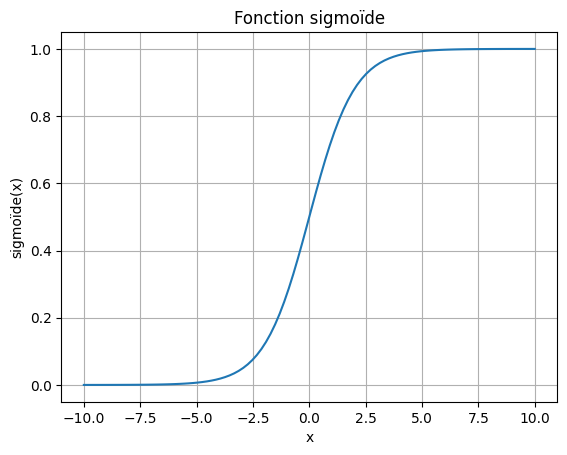
\includegraphics[width=0.6\textwidth]{f_sigmoide.png}
	 	\caption{La fonction sigmoïde}
	 	\label{fig:mesh1}
	 \end{figure}

	 Elle est l'inverse de la fonction LOGIT. Sa formule est :

 	\begin{equation}
 		\sigma(x) = \frac{1}{1 + e^{-x}}
 	\end{equation}

 	Où:
 	\begin{itemize}
 		\item $\sigma(x)$ représente la fonction sigmoïde
 		\item $e$ est la base du logarithme naturel (constante d'Euler)
 		\item $x$ est la variable d'entrée
 	\end{itemize}

 	Les deux fonctions logistique et LOGIT étant inverses l'une de l'autre, cela signifie que :
 	\begin{itemize}
 		\item $\text{logit}(\sigma(x)) = x$
 		\item $\sigma(\text{logit}(p)) = p$
	 \end{itemize}}

	 \label{fonction softmax}
	 \entreelex{Fonction softmax}{La fonction softmax est une fonction d'activation qui transforme un vecteur de nombres réels en une distribution de probabilités.}

	\entreelex{Modalité de référence}{Modalité de référence par rapport à laquelle le LOGIT est exprimé.}

	\label{taux apprentissag}
	\entreelex{Taux d'apprentissage}{Ou learning Rate : il fixe la « grandeur » du pas de chaque itération de la descente de gradient.}

	\listoffigures

    \printbibliography

\end{document}
